\section{Simulation}
\subsection{Switches}
Switches allow for the selective connection or disconnection of different loads while power is applied to the circuit. When it comes to resistive loads, they exhibit no dynamic response to changes in voltage or current. This implies that the ideal resistor model \eqref{eq:ideal_resistor} holds true.
\leavevmode\newline

In contrast, when dealing with \textit{inductive loads}, it is important that the current through the inductor ($I_L$) is zero at the time of connection for the derived equations to hold true. This is due to the property of inductors resisting changes in current. \citep{inductor}

\subsubsection{Considerations when Disconnecting Inductive Loads}
However, disconnecting an inductive load presents a different scenario. Here, an ideal switch is presumed, which disconnects instantaneously as $\Delta t$ tends to zero. Nevertheless, due to the inductive property of resisting changes in current, the current through the inductor will be non-zero at the instant of switching. This leads to an instantaneous reduction of current to zero, thus causing a voltage spike across the inductor according to Faraday's law: \citep{inductor2}

\begin{equation}
V_L = -L \frac{di}{dt}
\end{equation}

where $V_L$ is the voltage across the inductor, $L$ is the inductance, and $\frac{di}{dt}$ is the rate of change of current.

\subsubsection{Modelling Voltage Spike on Inductive Load Disconnection}

This spike, mathematically, approaches negative infinity, which is not physically meaningful. In reality, the voltage will increase abruptly, but the breakdown of the switch will eventually occur, leading to a non-instantaneous reduction of current. To model this scenario, the voltage across the diode in the cycle following the switch-off event is estimated as:

\begin{equation}
V_{L_{n+1}} = - \frac{L \cdot i_{n}}{h}
\end{equation}

where $V_{L_{n+1}}$ is the voltage across the inductor at the next cycle, $i_n$ is the current through the inductor at the current cycle, and $h$ is the time-step size.

\subsubsection{Post Disconnection of Inductive Load}
In the subsequent cycles after disconnection, the voltage and current across the inductor are both equal to zero. The voltage across the resistor will also be zero after the switch is flipped, since it is not a reactive element.

\pagebreak
\subsection{Algorithmic Implementation}
The numerical analysis of the circuit is implemented in MATLAB using the \texttt{powerSupply} function. This function applies the fourth-order Runge-Kutta method (RK4) to solve the governing differential equations.
\begin{itemize}
\item To manage varying load conditions, the design incorporates polymorphism by utilising four different sub-functions. Each sub-function handles the characteristic equations specific to a particular load condition.
\item RK4 is applied in each scenario to compute the state of the circuit at the next time step, based on the current state and input voltages (.i.e. determine the characteristic voltages and currents of the circuit)
\item The primary \small{\texttt{powerSupply}} function parses the \small{\texttt{mode}} argument to determine the current load condition. It then dispatches the calculation to the appropriate sub-function. This is managed through a switch-case control flow mechanism.
\item After obtaining the next state from the appropriate sub-function, \small{\texttt{powerSupply}} calculates the remaining circuit parameters, $i_c(t), i_z(t), i_s, i_d(t)$.
\end{itemize}
The code is organised modularly, separating the overall simulation flow from the specific equations for different load conditions. This structure makes the design robust, readable, maintainable, and easily extendable for additional load conditions or complexities.

\lstinputlisting[caption=Primary MATLAB function for simulating the power supply operations using RK4]{code/powerSupply.m}

\subsubsection{No Load Scenario}
\lstinputlisting[caption=Sub-function for the no-load scenario of the power supply simulation]{code/powerSupply_noLoad.m}

\subsubsection{Resistive Load Scenario}
\lstinputlisting[caption=Sub-function for the resistive load scenario of the power supply simulation]{code/powerSupply_resistiveLoad.m}

\subsubsection{Inductive Load Scenario}
\lstinputlisting[caption=Sub-function for the inductive load scenario of the power supply simulation]{code/powerSupply_inductiveLoad.m}

\subsubsection{Full Load Scenario}
\lstinputlisting[caption=Sub-function for the full-load scenario of the power supply simulation]{code/powerSupply_fullLoad.m}

\pagebreak
\subsection{Timestep Selection}
The time-step $h$ used in the RK4 method was determined using,
\begin{equation}
	h = \frac{T}{c}
\end{equation}
where $T$ is the period of the input sinusoid, or $0.02$  (corresponding to a 50 Hz signal), and $c$ is the desired number of samples per period (also known as the sampling rate).
\begin{itemize}
	\item A sensible choice for \(h\) would be sufficiently small to accurately capture the behavior of the system within each period of the sinusoidal input. Applying the Nyquist sampling theorem, \(c\) should be at least twice the highest frequency present in the signal to avoid aliasing. Therefore, a minimum value of \(c = 2 \times 50 = 100\) samples per second would be needed.
	\item However, for numerical solutions of differential equations using the RK4 method, we may require a higher sampling rate to capture the system dynamics more accurately. In this case, \(c\) could be set to a much larger value, leading to a smaller time step \(h\).
	\item For instance, setting \(c = 1000\) samples per second would result in a time step $h = \frac{0.02}{1000} = 20\mu s$, giving us a high-resolution representation of the system's behaviour within each period of the sinusoidal input.
\end{itemize}

A step size of $80\mu s$, $40 \mu s$ and $20 \mu s$, corresponding to a sampling rate of $250$, $500$ and $1000$ cycles per second (respectively) produced sensible results in the simulation across all loads. $40 \mu s$ was chosen as the final value which offered a reasonable compromise between computation time and quality of results. 

\pagebreak
\subsection{Results}
The results of the simulation with a time step of $h = 40 \mu s$ are shown across all four load conditions. Each respective plot shows the voltages at node \textcircled{2} and \textcircled{3} alongside the inductor $i_l(t)$ and zener $i_z(t)$ currents, with respect to time.

\subsubsection{No Load}
\begin{figure}[H]
    \centering
    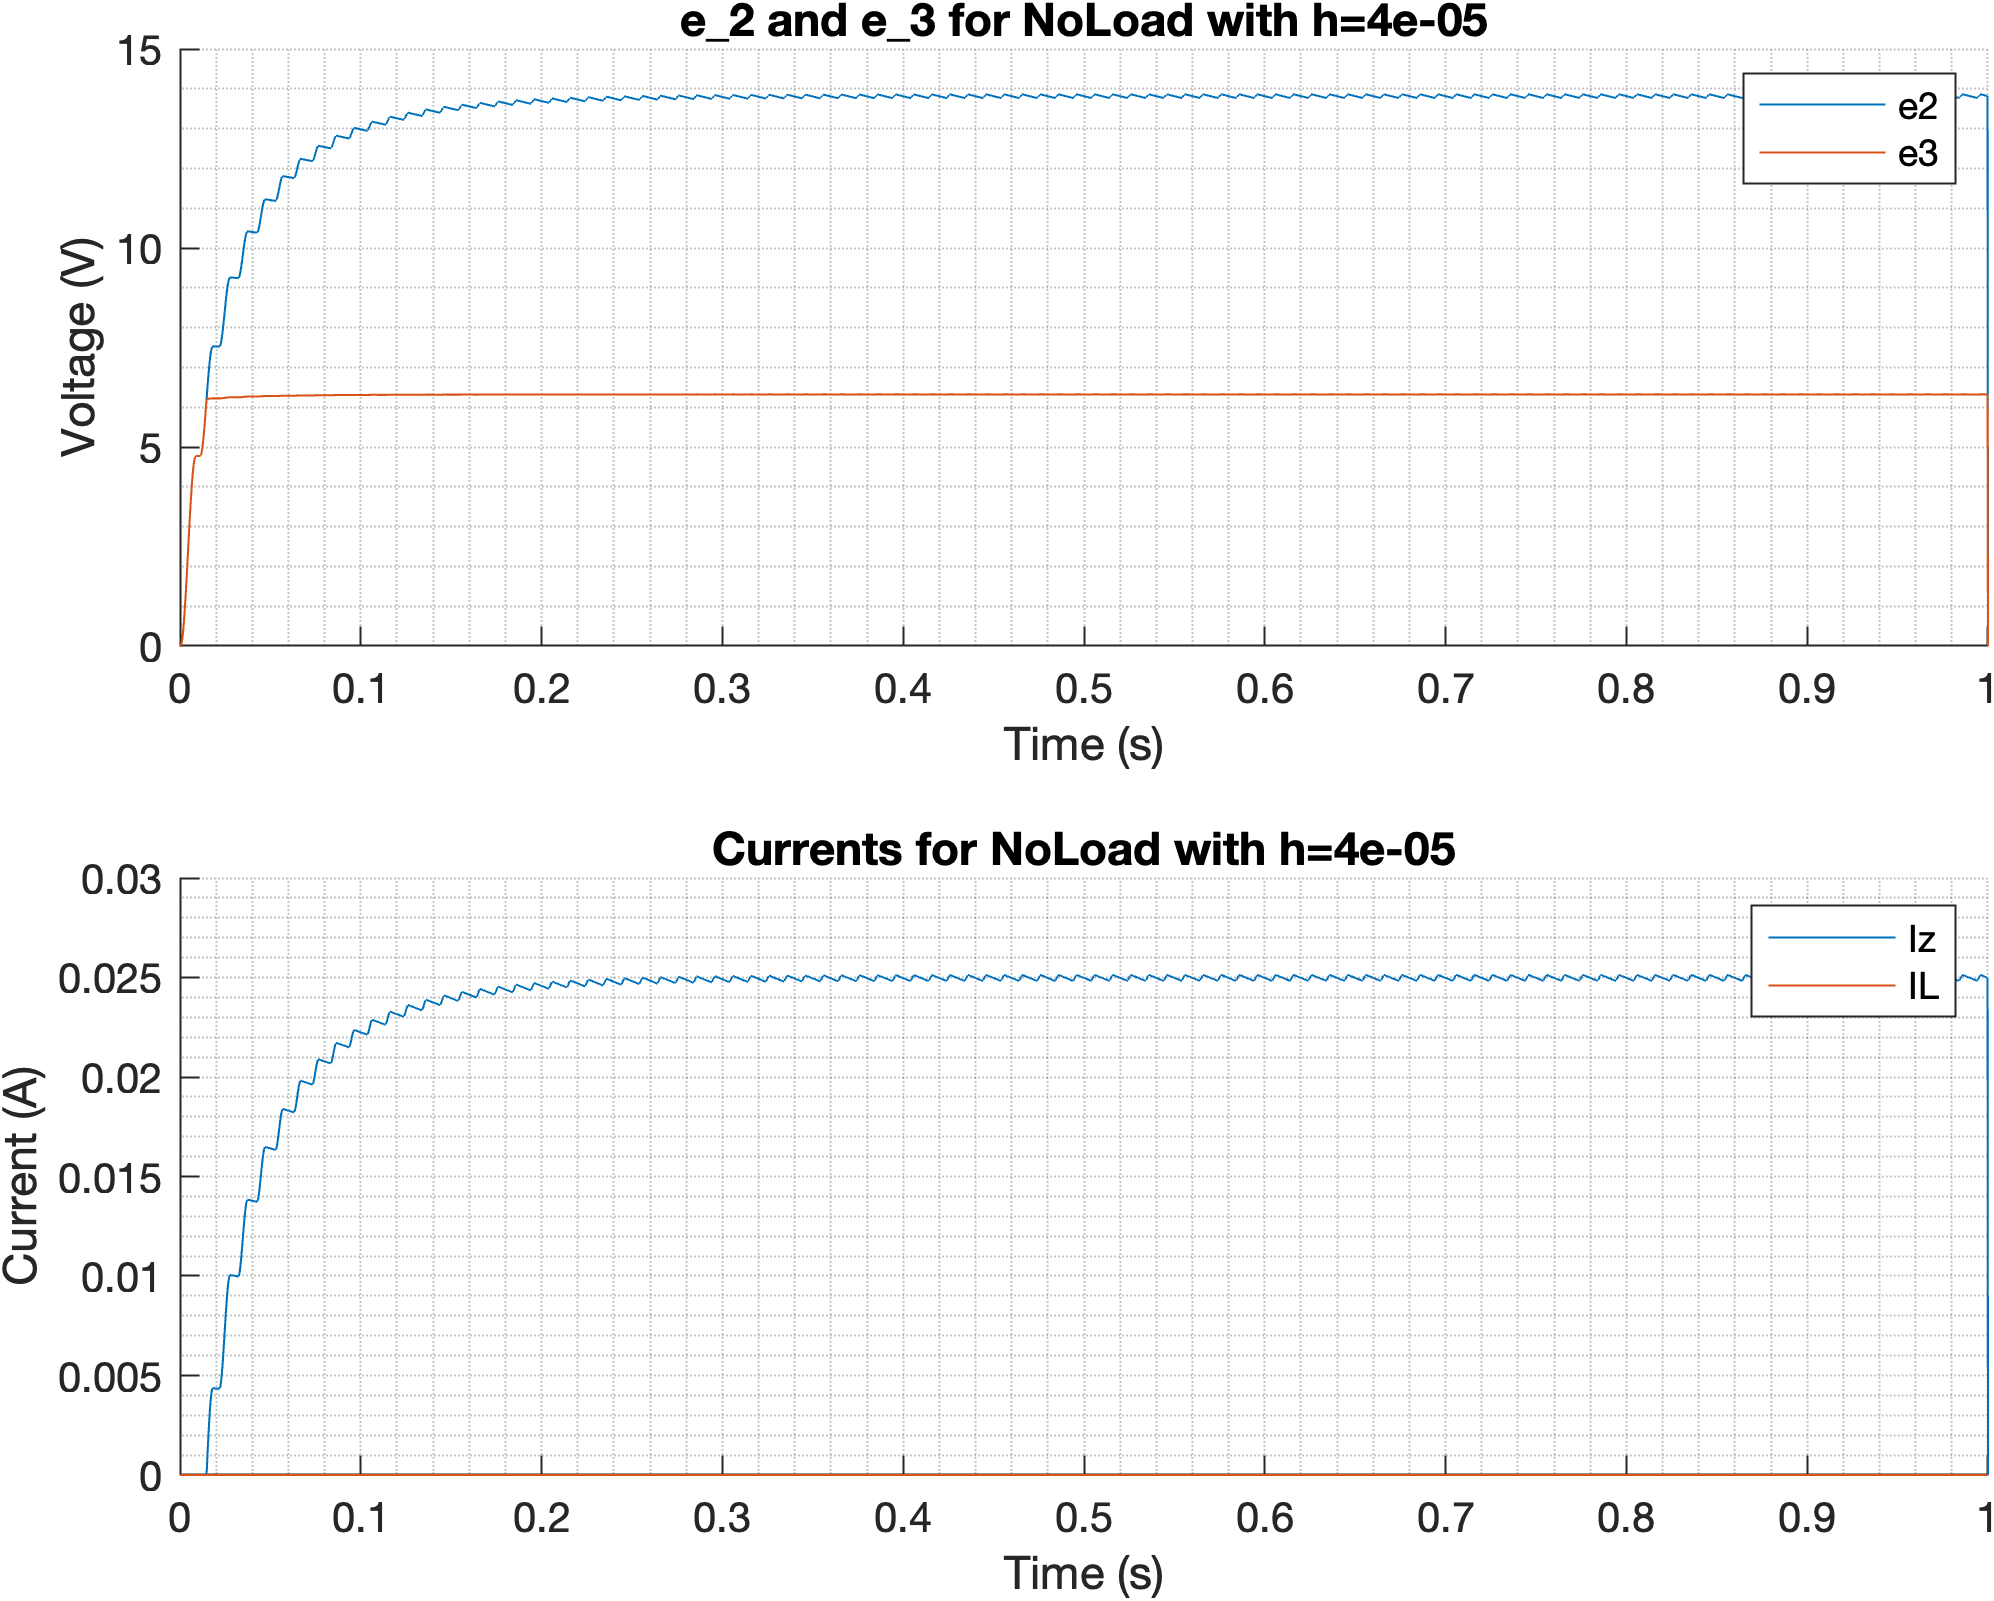
\includegraphics[width=\textwidth]{/graphics/exports/psp_NoLoad_h_4e-05.png}
    \caption{Node voltages and currents under no load conditions with $h=40\mu s$}
\end{figure}
\begin{itemize}
\item The node voltage $e_2$ reaches steady state at around $\approx 13.7V$ after a short duration of time.
\item Without any load connected to the circuit, the output voltage $e_3$ mirrors the input voltage at node \textcircled{2} until it reaches the zener reverse breakdown voltage at around $\approx 6.1V$.
\item After this point, the Zener diode enters reverse breakdown and begins conducting. Thus, the output voltage is regulated and reaches steady state at this level.
\item The current $I_l$ remains at zero throughout the simulation as no inductive load is connected to the circuit. The zener current $I_z$ reaches steady state when the zener is in reverse breakdown and remains at zero when the zener is in cut off.
\end{itemize}

\subsubsection{Inductive Load}
\begin{figure}[H]
    \centering
    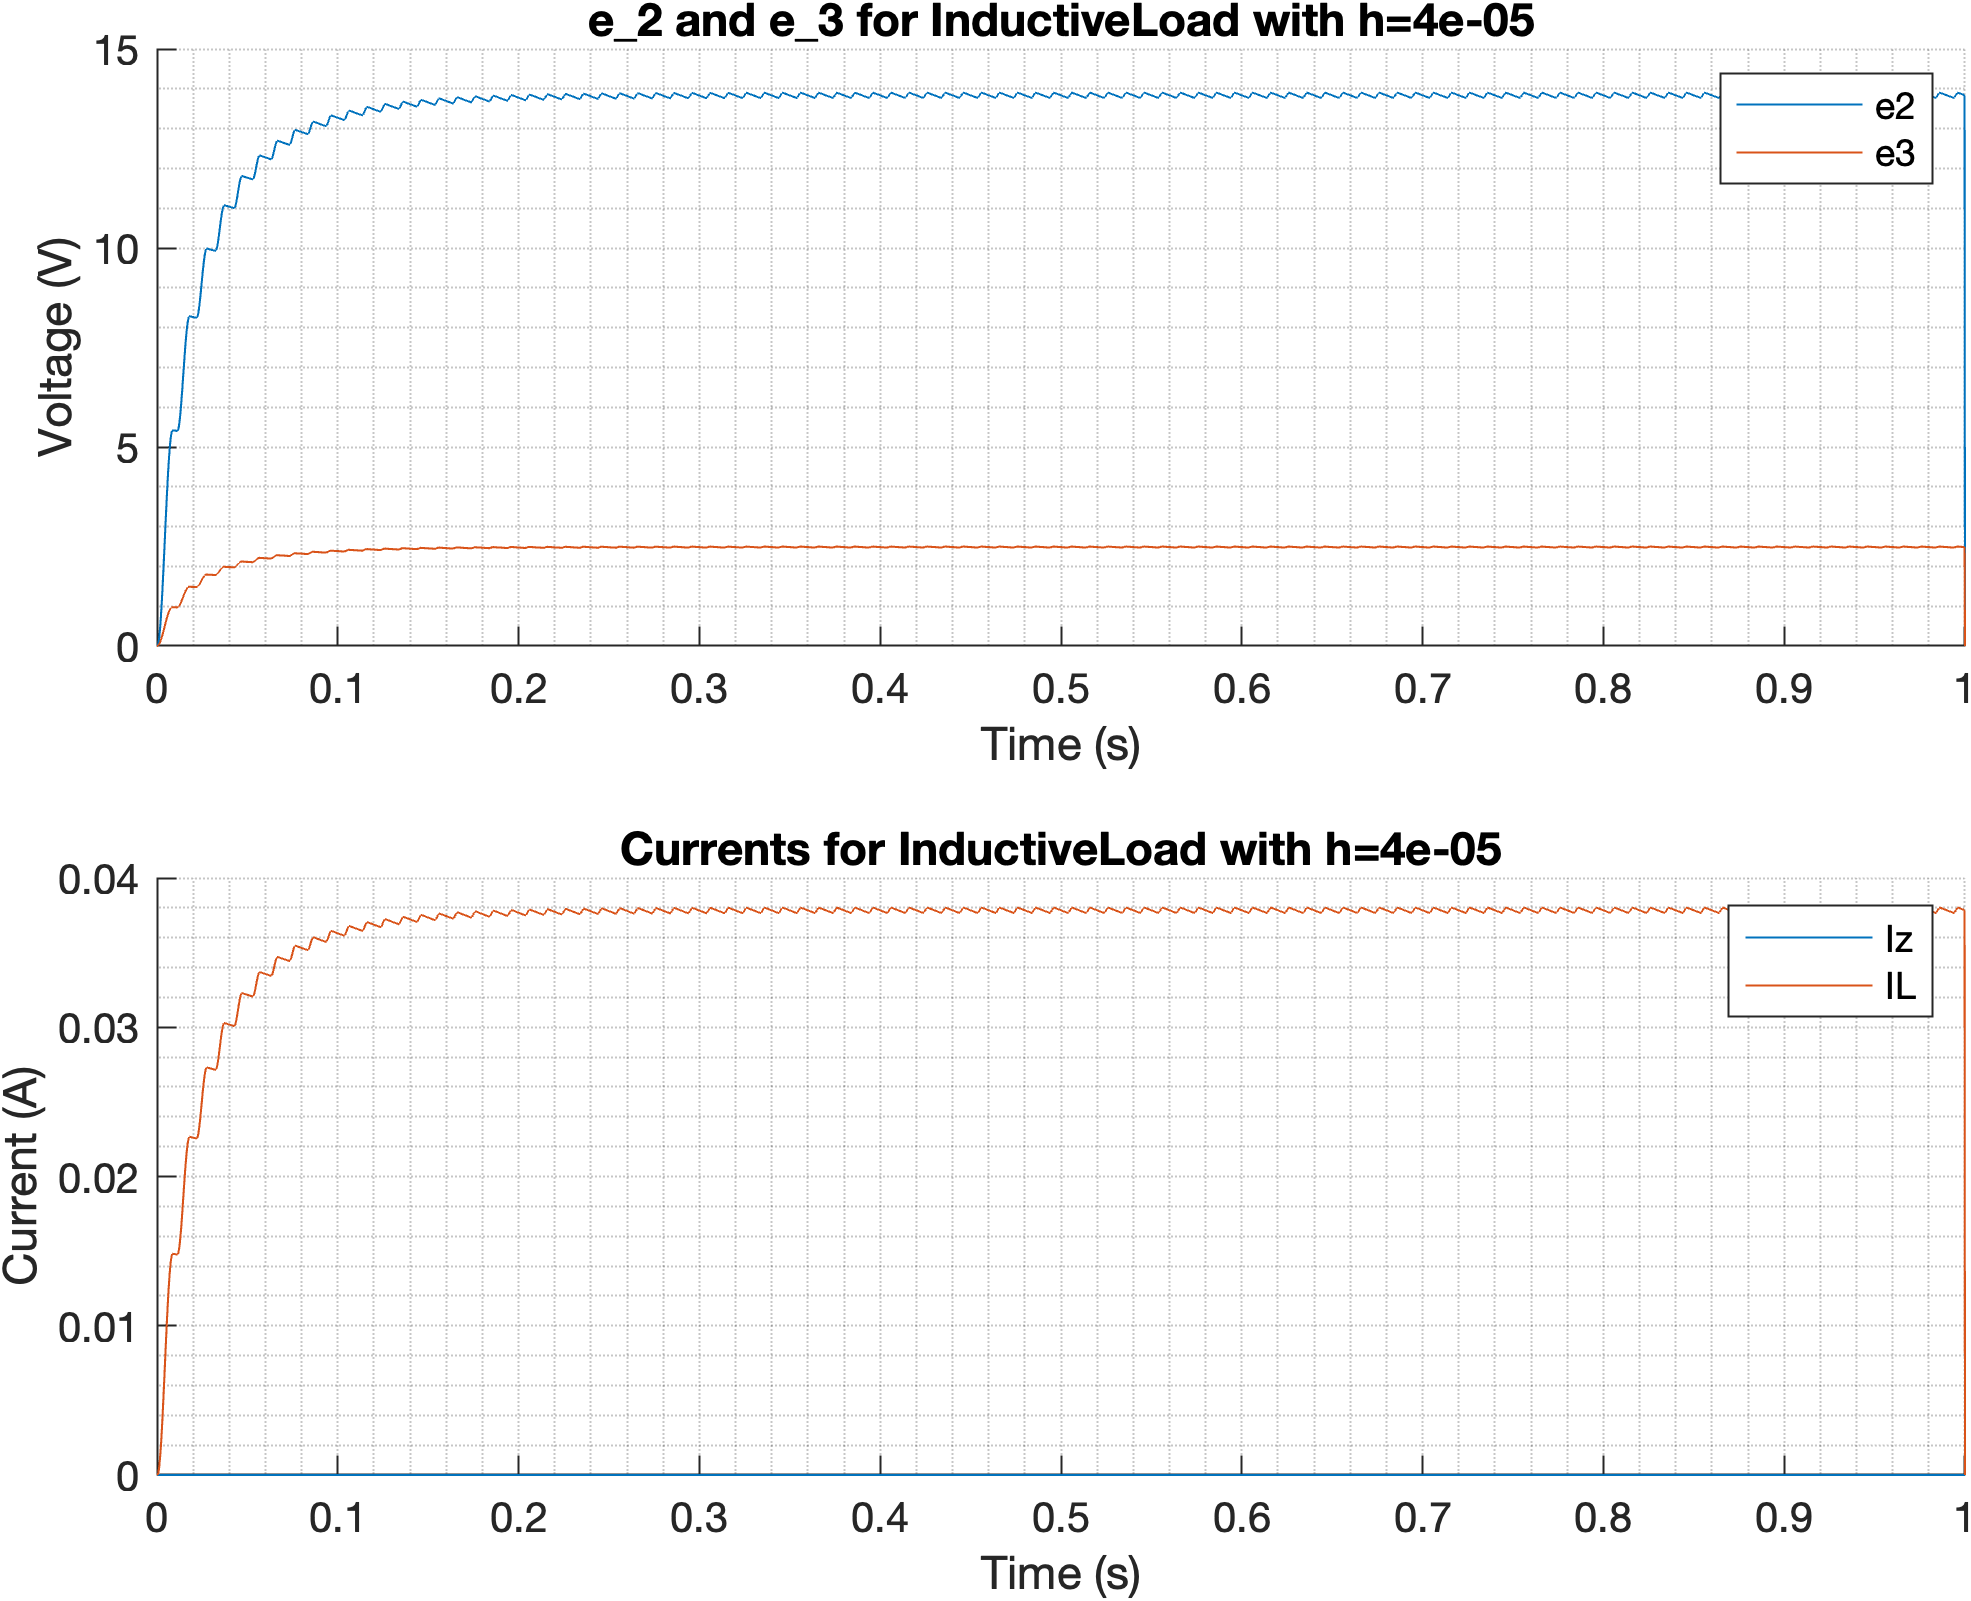
\includegraphics[width=\textwidth]{/graphics/exports/psp_InductiveLoad_h_4e-05.png}
    \caption{Node voltages and currents under Inductive Load conditions with $h=40\mu s$}
\end{figure}
\begin{itemize}
	\item With an inductive load, the node voltage $e_2$ is unaffected and remains in steady state of $\approx 13.7V$ after a short duration of time
	\item The node voltage $e_3$ is significantly reduced, at about half of its value from no load conditions. This is because the added inductor and resistor draw additional current from the source, leading to an increase in the voltage drop across these components.
	\item The incorporation of the inductor and resistor in the circuit leads to a redistribution of voltage and current in the system. The inductor and resistor form a resistive-inductive (RL) load which has a characteristic impedance. This impedance draws more current from the source, thus reducing the voltage at node $e_3$.
	\item The zener acts as an open circuit as $e_3$, as is below the threshold voltage $V_z$, and is in cut off. Thus, no current flows through the `ener diode, keeping the current level $I_z$ at zero.
\end{itemize}

\subsubsection{Resistive Load}
\begin{figure}[H]
    \centering
    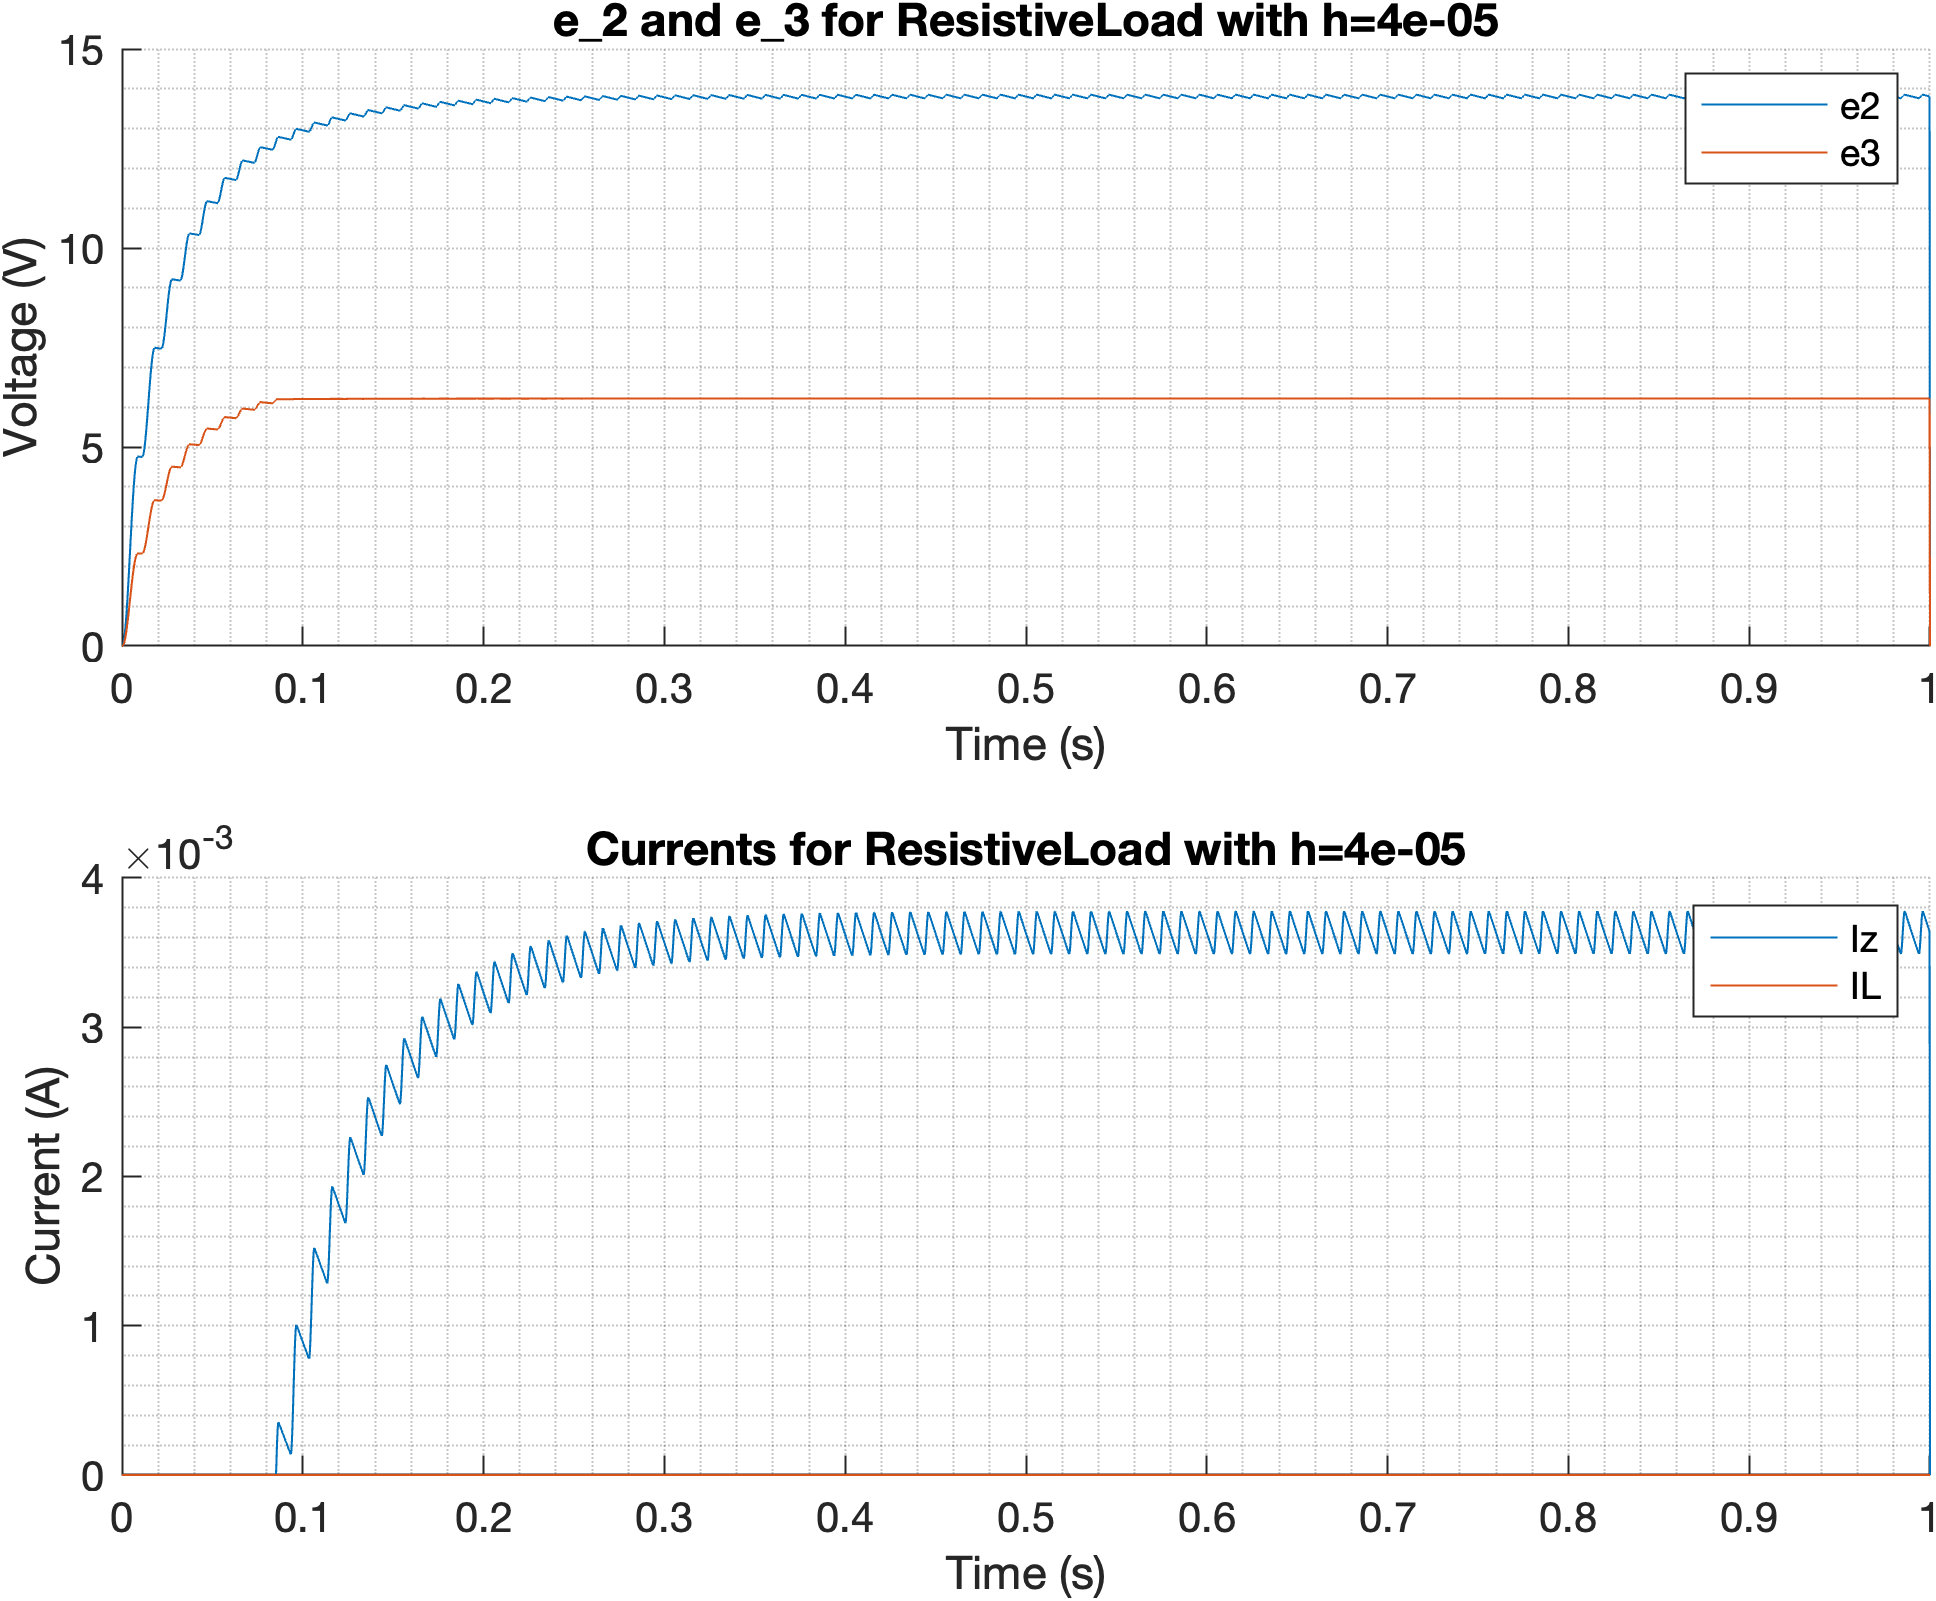
\includegraphics[width=\textwidth]{/graphics/exports/psp_ResistiveLoad_h_4e-05.png}
    \caption{Node voltages and currents under resistive load conditions with $h=40\mu s$}
\end{figure}
\begin{itemize}
\item When a resistive load is present, the node voltage $e_2$ maintains its steady state at approximately $13.7V$ after a short period of time.
\item Similar to the case without any load, the output voltage $e_3$ saturates around the reverse breakdown voltage of the zener diode, approximately $6.1V$.
\item At this threshold, the zener diode switches from cutoff to reverse breakdown and starts functioning as a voltage regulator within the circuit. The zener current $I_z$ remains at zero initially but reaches a steady state shortly after this transition.
\item Since there is no inductive load connected, the current through the inductive branch, $I_l$, remains at zero.
\item The presence of the resistor in parallel with the zener diode causes a significant reduction in the steady state zener current $I_z$ compared to the case without any load.
\end{itemize}

\subsubsection{Full Load}
\begin{figure}[H]
    \centering
    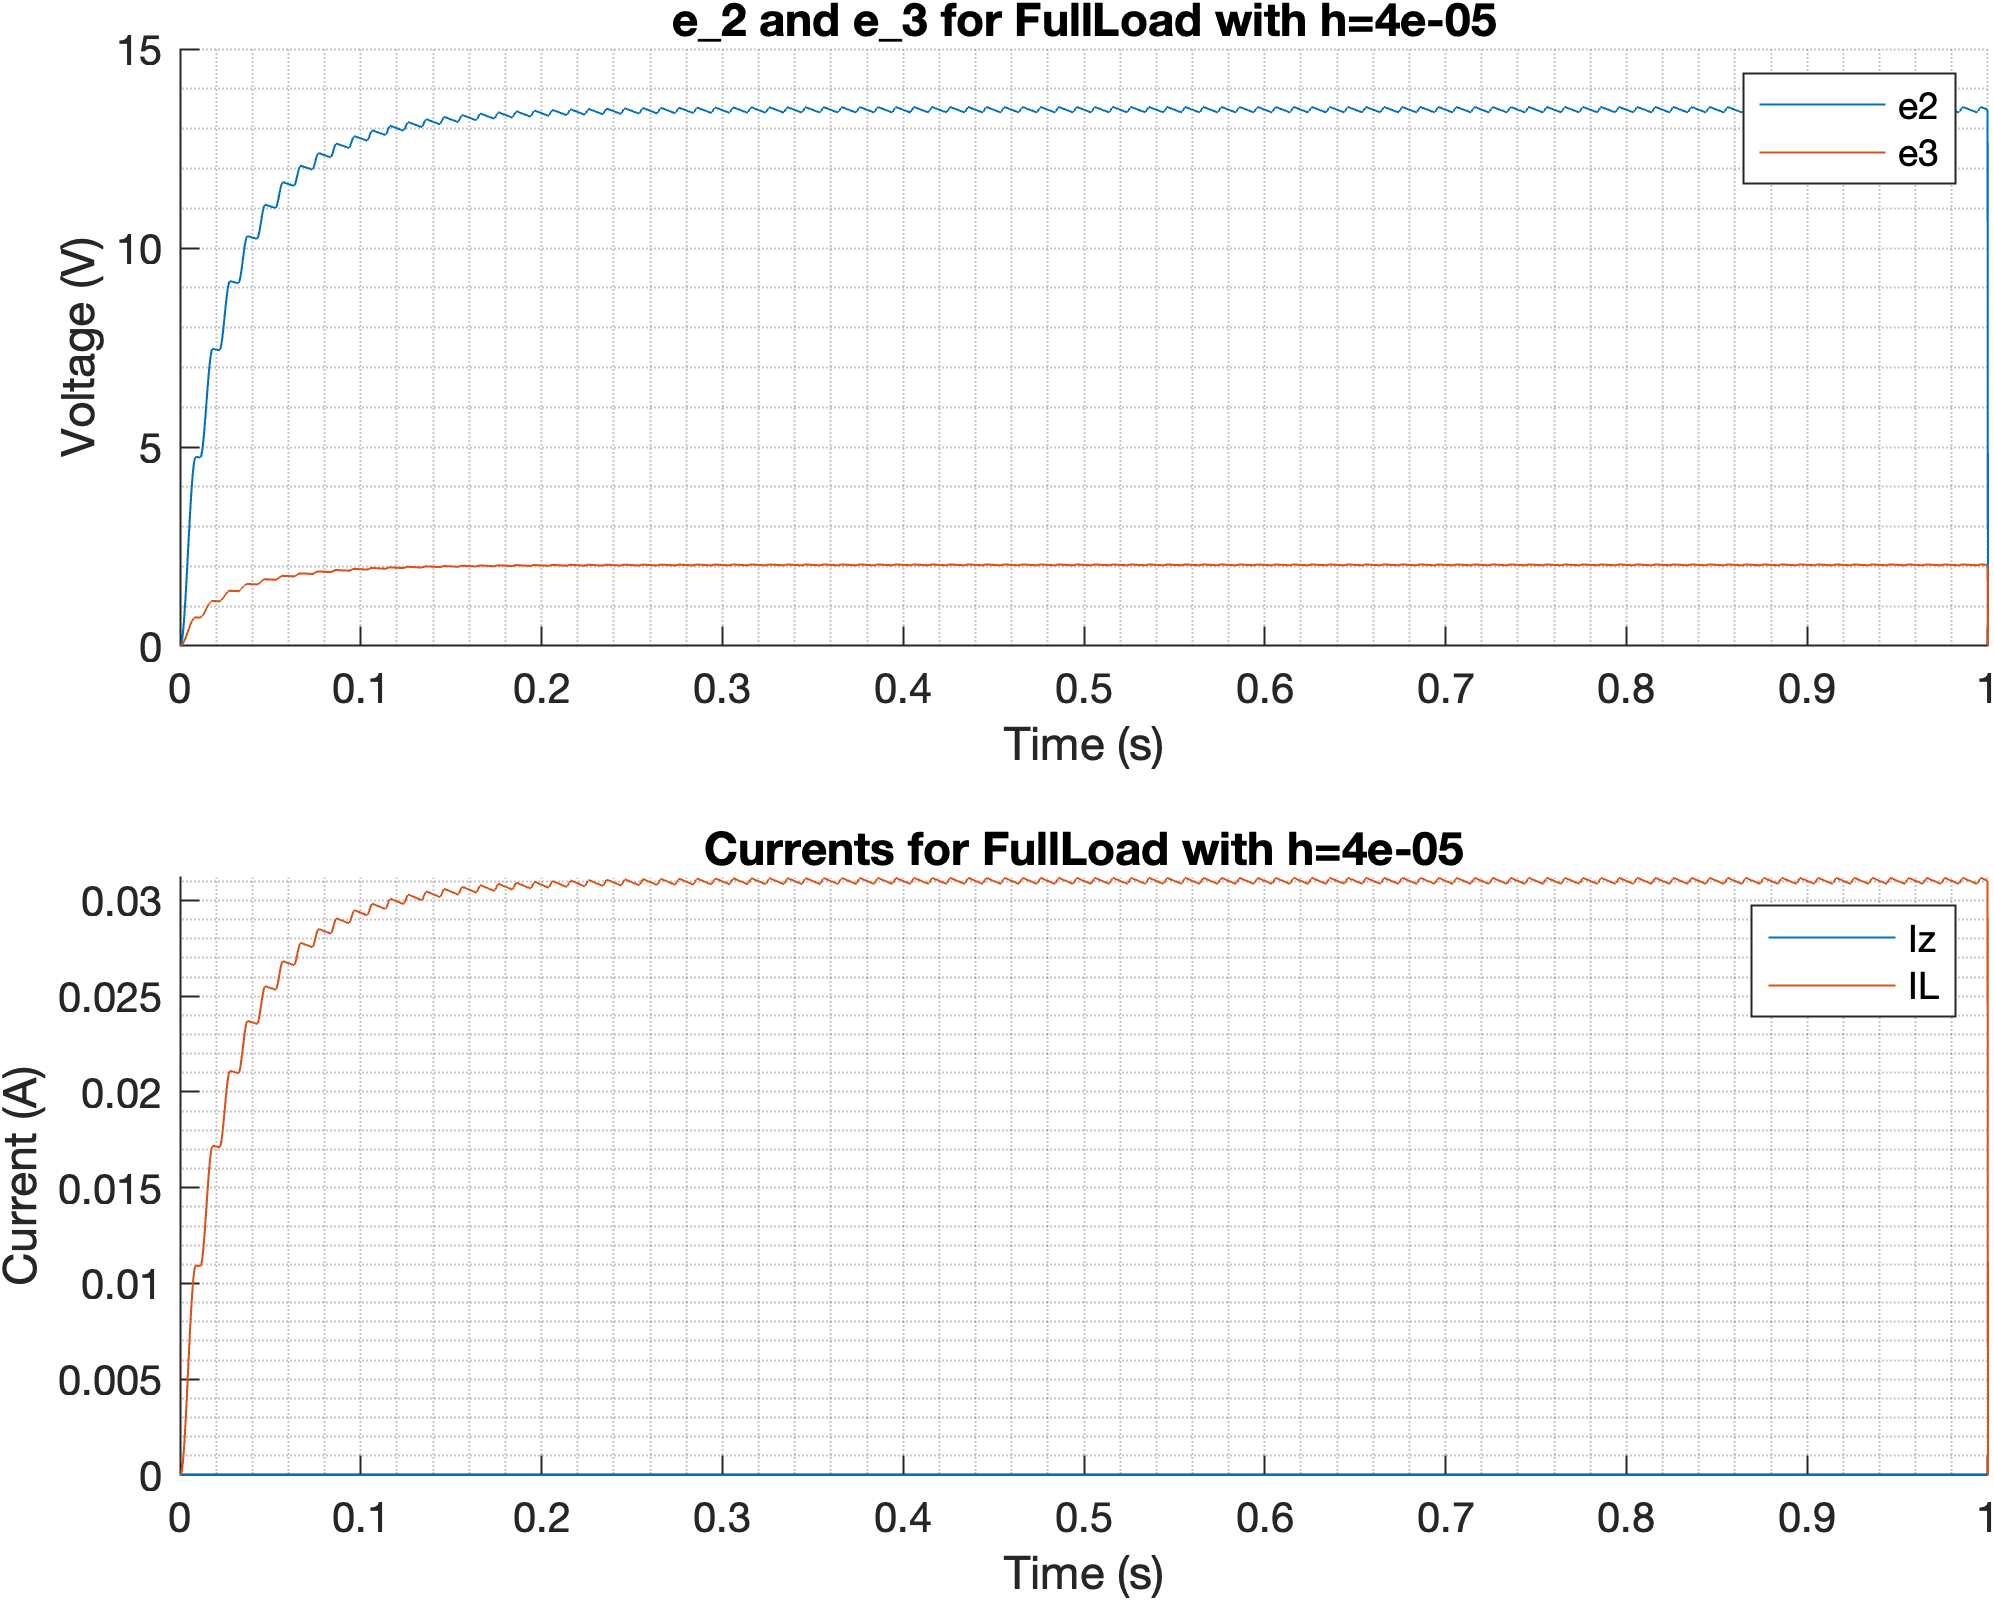
\includegraphics[width=\textwidth]{/graphics/exports/psp_FullLoad_h_4e-05.png}
    \caption{Node voltages and currents under Full Load conditions with $h=40\mu s$}
\end{figure}
\begin{itemize}
	\item With a full load (.i.e. inductive and resistive) connected to the circuit, the node voltage $e_2$ again remains unaffected. It reaches steady state at $\approx 13.7V$ after a short duration of time.
	\item The output voltage $e_3$ is significantly reduced in this scenario, furthermore than in the inductive load case. 
	\item With the addition of a resistive load in parallel to the inductive-resistive series load, the overall impedance of the load decreases. This is due to the parallel resistor offering an alternate path for the current to flow, which increases the total current in the circuit.
	\item This increased current flow results in a higher voltage drop across the series-connected resistor and inductor, leading to a further decrease in node voltage $e_3$. Even in steady state, the inductor in this configuration will not behave as a short circuit because the alternating current will keep flowing through the parallel resistive branch.
	\item Throughout the simulation, the zener diode remains in the cut-off region due to the truncation of the node voltage $e_3$ before it reaches the reverse breakdown region. Consequently, $I_z=0$
\end{itemize}

\pagebreak
\subsection{Maximum Diode Current}
In Section \ref{determinationOfMaximimumCurrent}, the maximum current flowing through the diodes was estimated to be $\simeq 1.917A$.The simulated diode current across all modes of operation is plot for 8 cycles of the input voltage $V_{in}(t)$:
\begin{figure}[H]
	\centering
	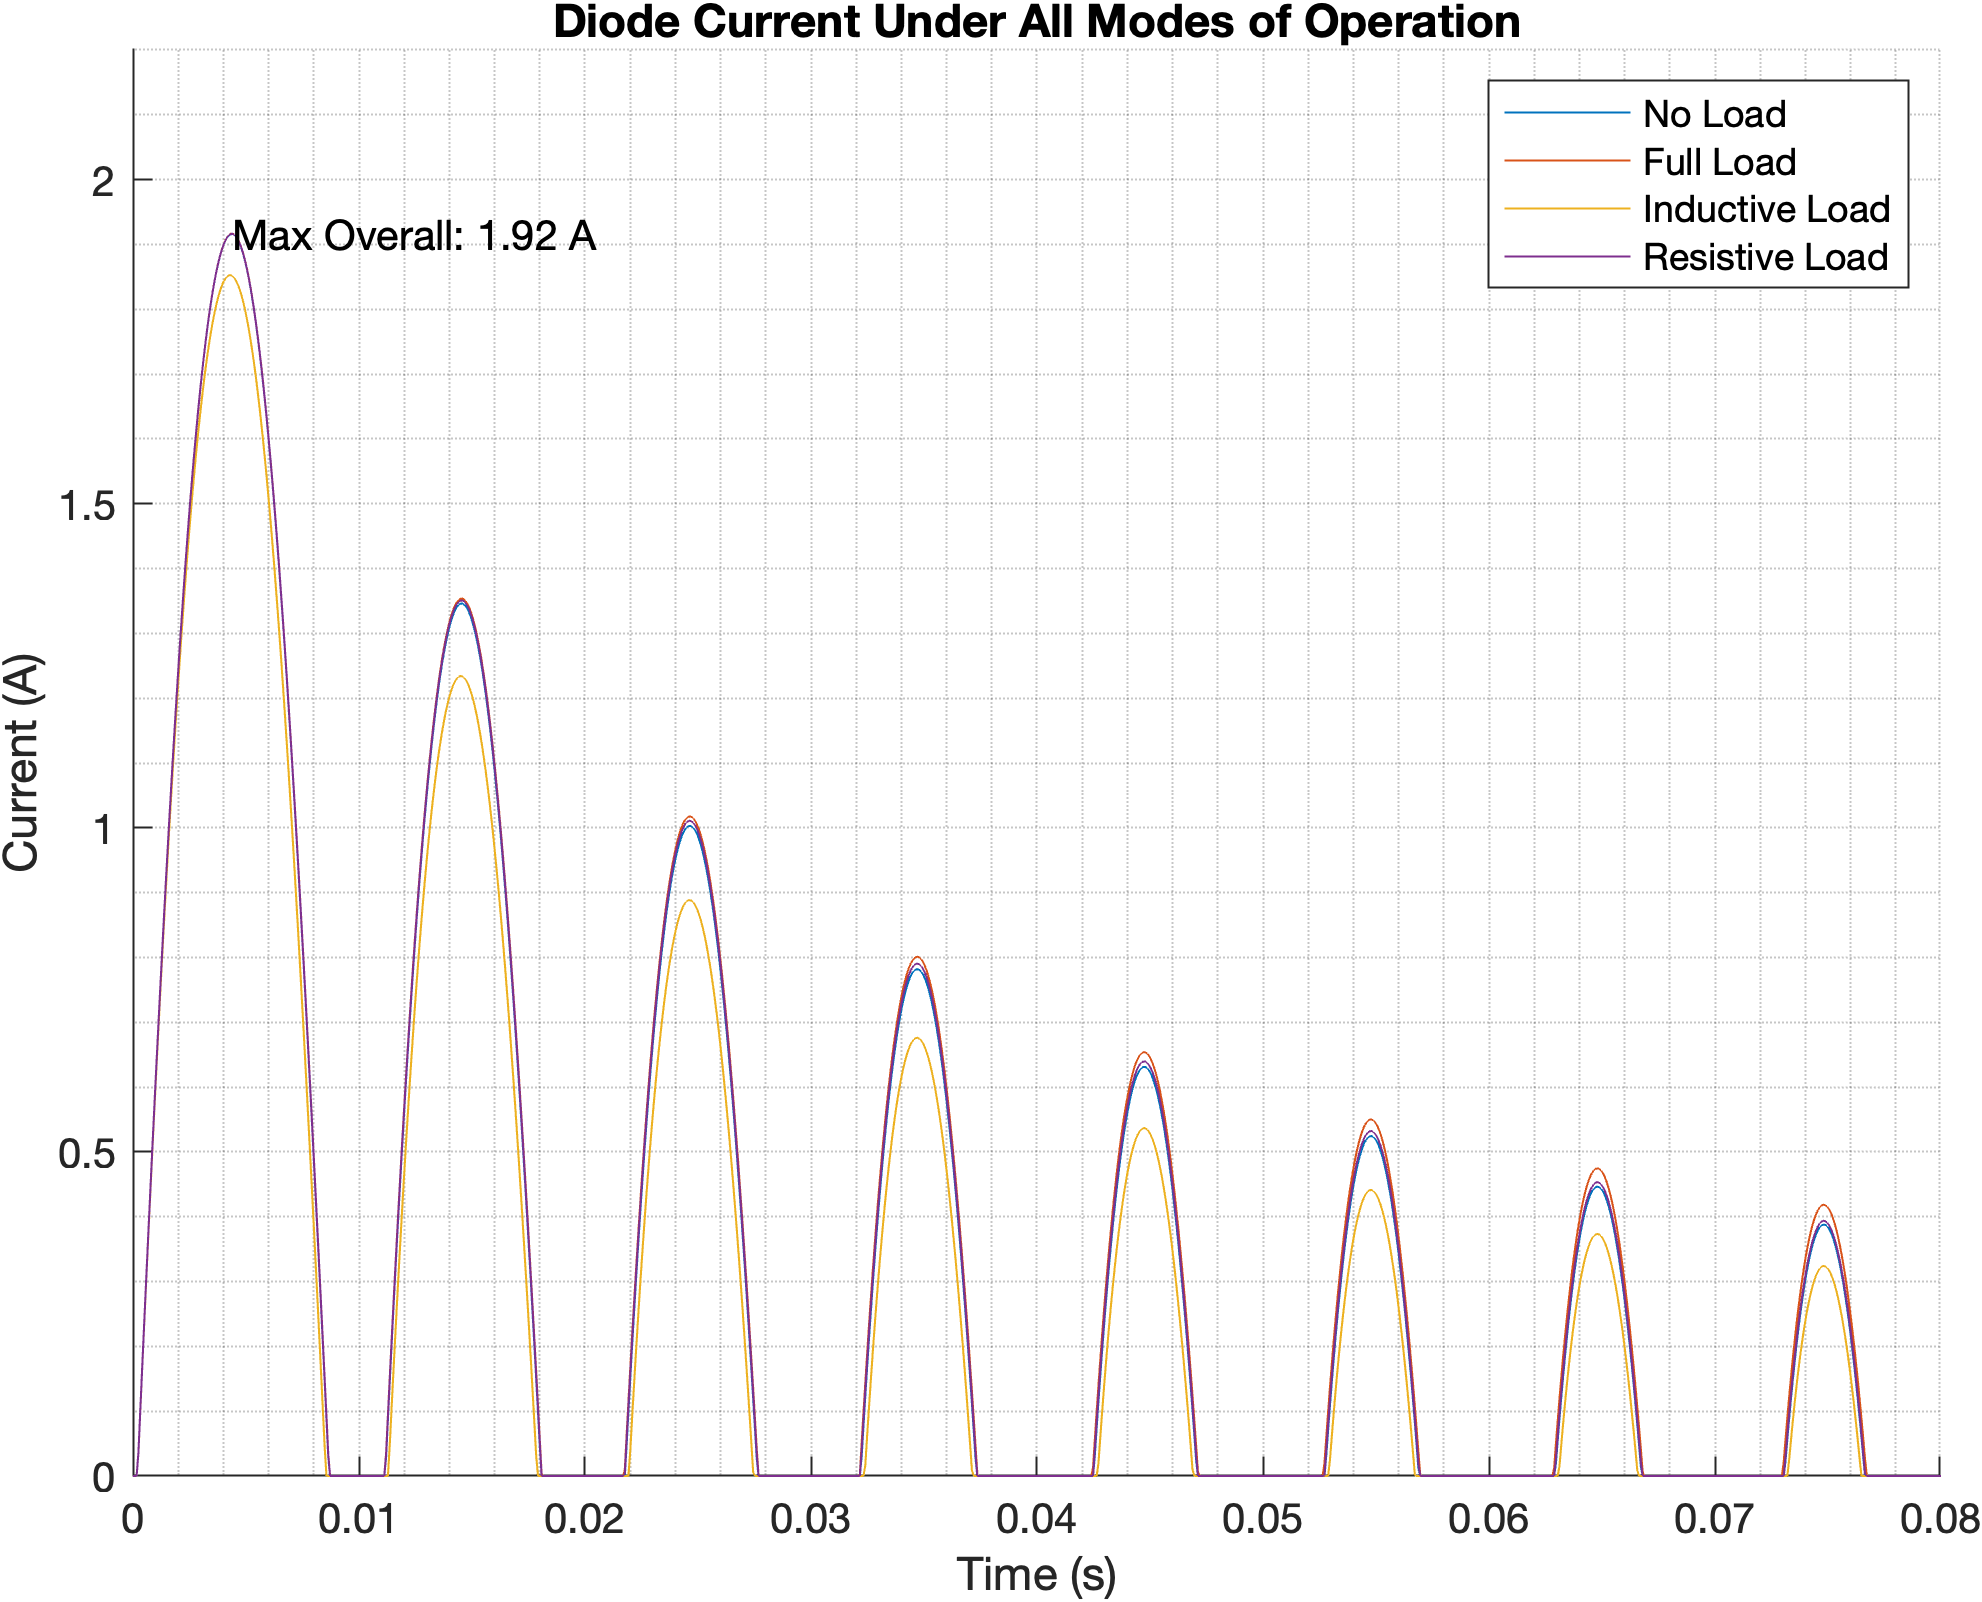
\includegraphics[width=\textwidth]{/graphics/exports/diode_current_MIN.png}
	\caption{Maximum diode in the circuit across all modes of operation}
\end{figure}

\begin{itemize}
	\item The maximum current flowing through the diode occurs $t \simeq 0$. This supports the initial assumption made in section \ref{determinationOfMaximimumCurrent}, that the peak current occurs during the first half cycle.
	\item The simulated maximum was $1.92A$ which approximately equals the analytically derived $1.917A$. 
	\item This validates the piece-wise linear approximation of the ideal diode that was made during the modelling of the circuit, and shows that our estimation was very reasonable. 
\end{itemize}

\pagebreak
\subsection{Power Dissipation in $R_s$}
Resistor $R_s$ has a tolerance of $\pm 10\%$ and a maximum power rating of $0.5W$. The power dissipated across resistor $R_s$ must not exceed this rating across all modes of operation. The power is be determined using $P=VI$ and applying Ohm's law such that
\begin{equation}
	P=R_sI_s^2
\end{equation}
The power dissipation was simulated for all four modes of operation with respect to time, for $R_s = [270\Omega, 300\Omega, 330\Omega]$. The maximum power does not exceed the $0.5W$ rating at any point during the simulation, across all four modes with the three possible values of $R_s$.  The results are detailed below

\subsubsection{Minimal Resistance}
\begin{table}[H]
\centering
\begin{tabular}{|c|c|}\hline
	\textbf{Mode of Operation} & \textbf{Maximum Power Dissipated (W)} \\\hline
	No Load & 0.17W \\
	Full Load &  0.17W \\
	Inductive Load & 0.39W \\
	Resistive Load & 0.40W \\\hline
\end{tabular}
\caption{Maximum power dissipated in $R_s$ with $R_s = 270\Omega$ across all four modes}
\end{table}
\begin{figure}[H]
	\centering
	\includegraphics[width=14cm]{/graphics/exports/power_dissipation_min.png}
	\caption{The power dissipated in $R_s$ with $R_s = 270\Omega$ across all four modes}
\end{figure}

\subsubsection{Nominal Resistance}
\begin{table}[H]
\centering
\begin{tabular}{|c|c|}\hline
	\textbf{Mode of Operation} & \textbf{Maximum Power Dissipated (W)} \\\hline
	No Load & 0.19W \\
	Full Load &  0.19W \\
	Inductive Load & 0.43W \\
	Resistive Load & 0.44W \\\hline
\end{tabular}
\caption{Maximum power dissipated in $R_s$ with $R_s = 300\Omega$ across all four modes}
\end{table}
\begin{figure}[H]
	\centering
	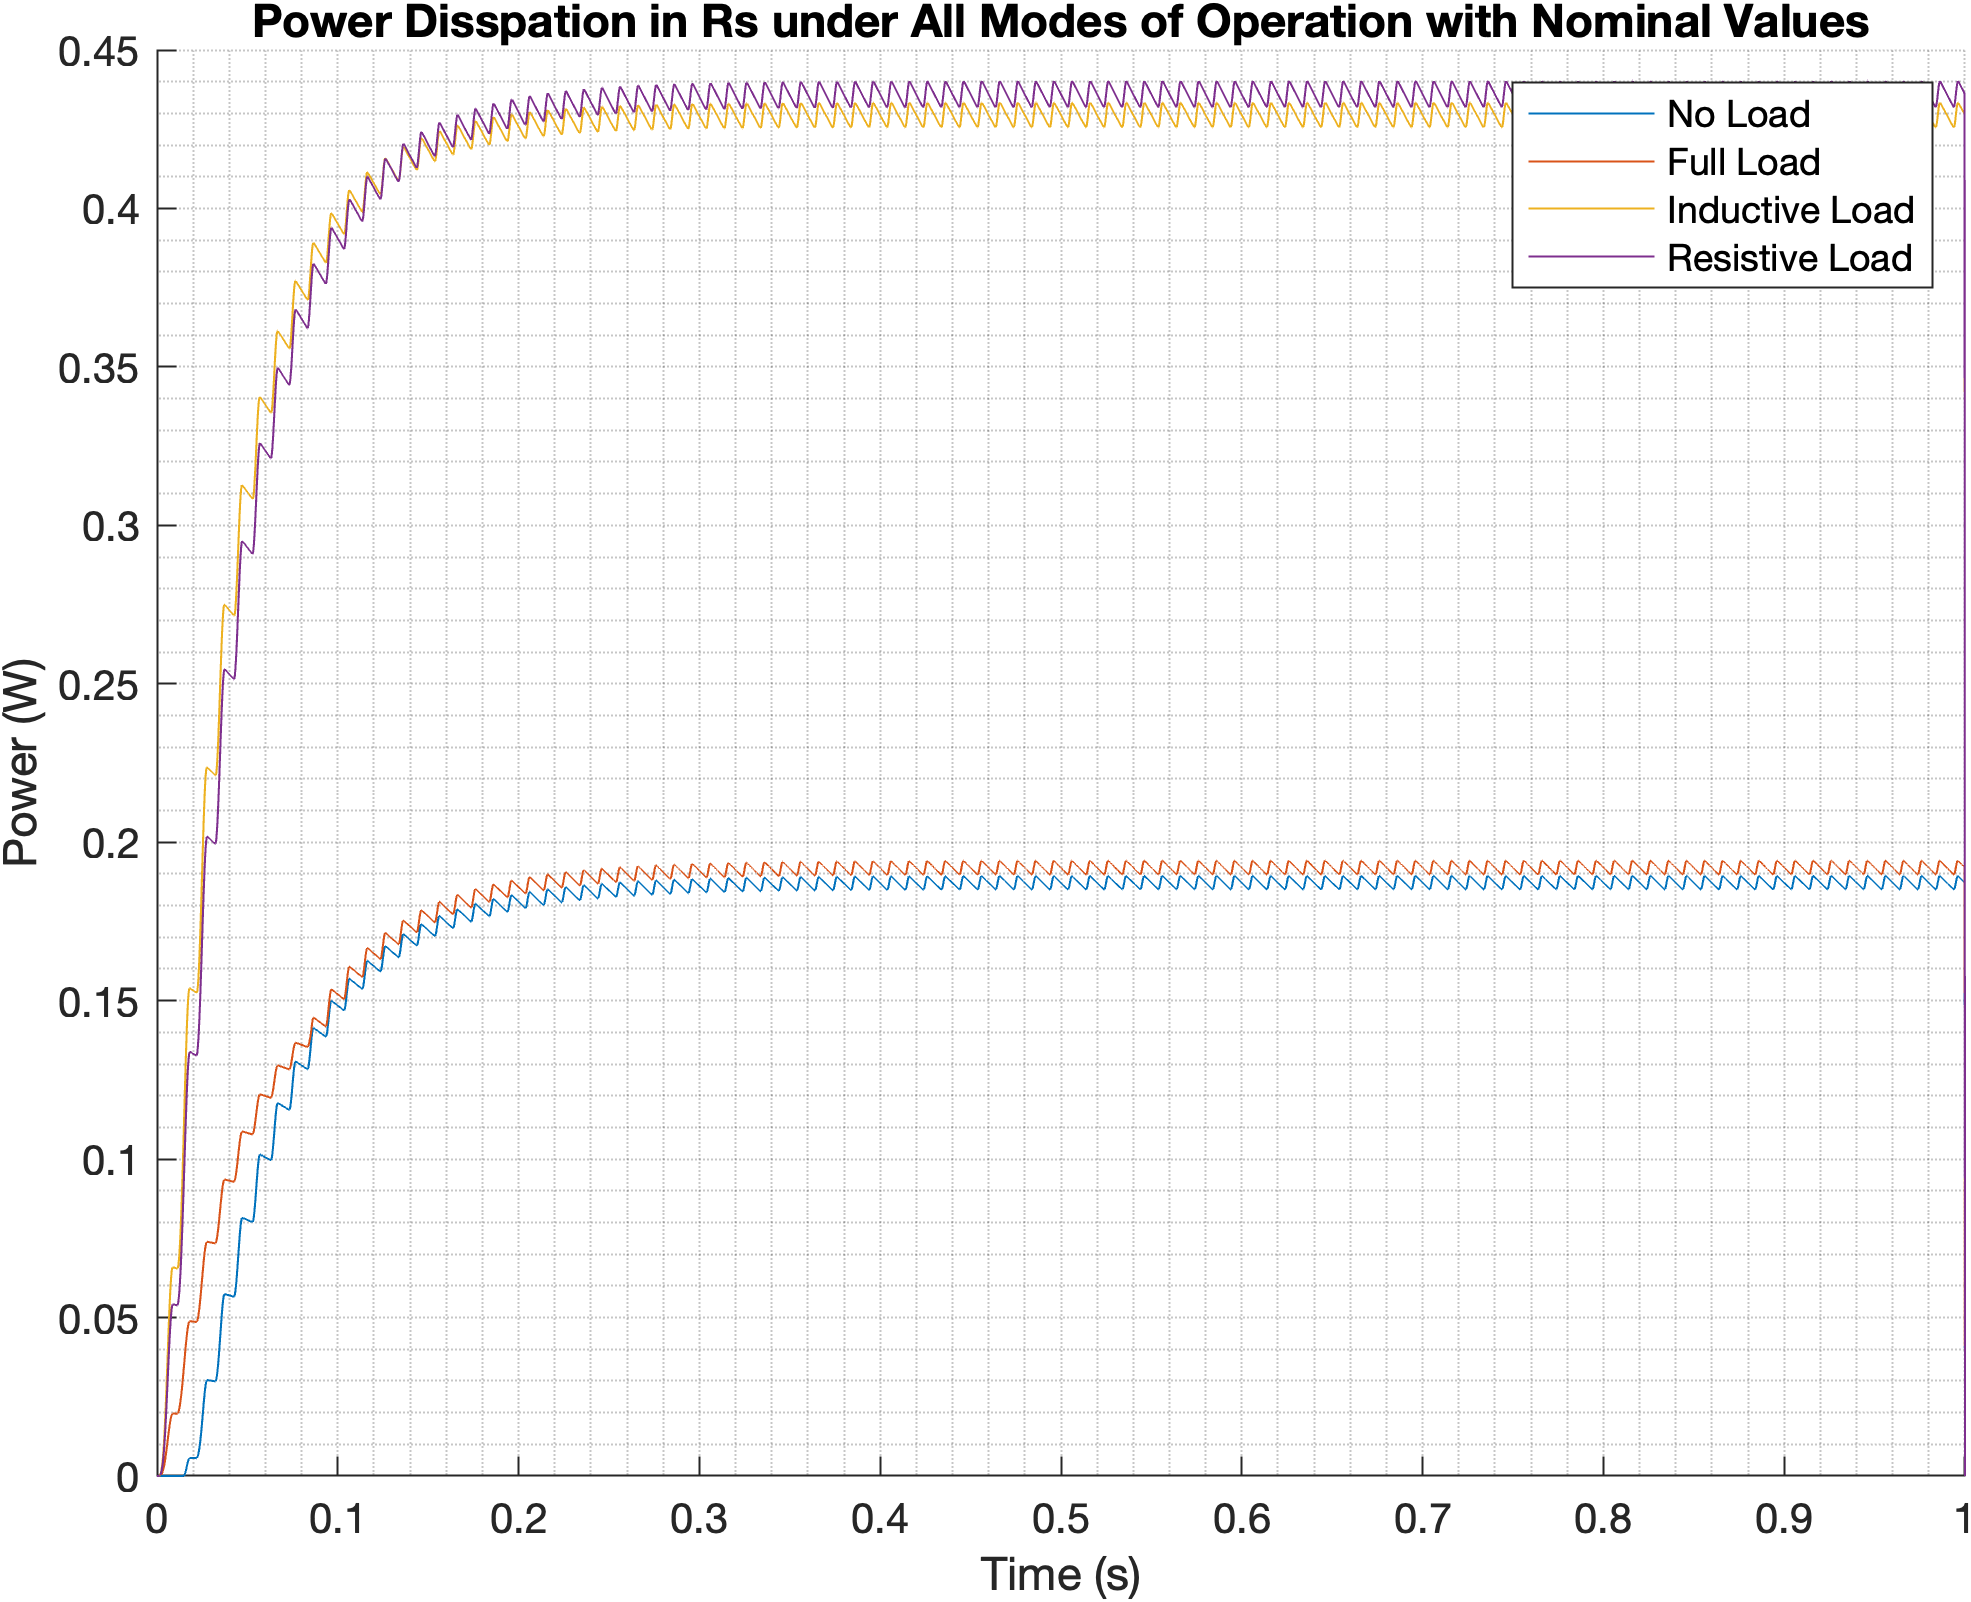
\includegraphics[width=14cm]{/graphics/exports/power_dissipation_nominal.png}
	\caption{The power dissipated in $R_s$ with $R_s = 300\Omega$ across all four modes}
\end{figure}

\subsubsection{Maximal Resistance}
\begin{table}[H]
\centering
\begin{tabular}{|c|c|}\hline
	\textbf{Mode of Operation} & \textbf{Maximum Power Dissipated (W)} \\\hline
	No Load & 0.21W \\
	Full Load &  0.21W \\
	Inductive Load & 0.48W \\
	Resistive Load & 0.48W \\\hline
\end{tabular}
\caption{Maximum power dissipated in $R_s$ with $R_s = 330\Omega$ across all four modes}
\end{table}

\begin{figure}[H]
	\centering
	\includegraphics[width=14cm]{/graphics/exports/power_dissipation_max.png}
	\caption{The power dissipated in $R_s$ with $R_s = 330\Omega$ across all four modes}
\end{figure}